\chapter{Engineering method}

Intro to what will be discussed in this chapter?

\section{Modularity}

Modularity is when legos

\subsection{Granularity}

Granularity is the average? Size of the module community

\subsection{Module families}

A collection of modules that can be treated as a singular module

\section{Tech Stack}

Started with Rust, because a \textit{low-level} language was assumed to be
necessary, to facilitate ease of C integration, which would allow for an
extendable application, which was language agnostic.

\section{Architecture}

% TODO: Some explanation on why this is an issue
% Also talk about what we tried first

\subsection{Module V.1}


First attempt was to create a Visual Studio Code Copy. This would've worked, but
would've created a lot of extra work.


\begin{itemize}
  \item First plan

    \begin{enumerate}
      \item Create an IDE

      \item Extend the IDE, to allow for a module architecture

      \item Modules call the application using some DSL

    \end{enumerate}
  \item Pros

    \begin{itemize}
      \item \textit{Easy} to implement

      \item Get a good understanding of what features might be needed

    \end{itemize}
  \item Cons

    \begin{itemize}
      \item Not really modular

      \item Will be subpar compared to existing software
    \end{itemize}
\end{itemize}

\subsection{Module V.2}


\begin{itemize}
  \item Second plan

    \begin{enumerate}
        % TODO: Add footnote
      \item Everything* is a module
    \end{enumerate}

    \begin{itemize}
      \item A module exposes three functions, that are invoked by the core

        \begin{itemize}
          \item Init - Returns a set of fields, which are added to the core state

          \item Update - Returns a set of fields which are updated

          \item View - Returns a set which represents HTML, which is rendered by
            the Core
        \end{itemize}

      \item Pros

        \begin{itemize}
          \item Easy to keep modules pure

          \item Optimization is possible due to the pureness of modules

          \item Easy to reason about module cooperation
        \end{itemize}

      \item Cons

        \begin{itemize}
          \item State is append-only

          \item State can only grow

          \item Not really modular
        \end{itemize}
    \end{itemize}
\end{itemize}

\begin{minted}{haskell}
data Value
  = VInt Int
  | VStr String
  | VBool Bool
  | VFloat Float
  | VLst [Value]
  | VObj [(String, Value)]

newtype State = [(String, Value)]
\end{minted}



\begin{minted}{haskell}
data Value
  = VInt Int
  | VStr String
  | VBool Bool
  | VFloat Float
  | VLst [Value]
  | VObj [(String, Value)]

newtype Map = [(String, Value)]

data Msg = Msg
  { msg :: String
  , val :: Value
  }
\end{minted}




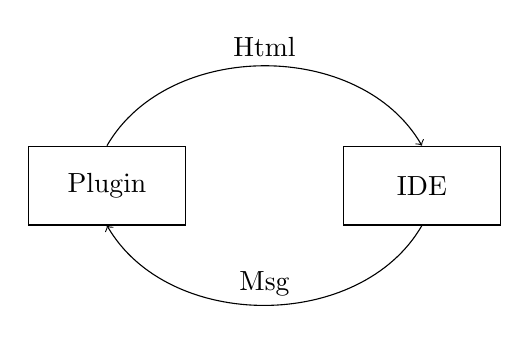
\begin{tikzpicture}
  % Nodes
  \node (p) [rectangle, draw, minimum height=1cm, minimum width=2cm] at (0, 0) {Plugin};
  \node (i) [rectangle, draw, minimum height=1cm, minimum width=2cm] at (4, 0) {IDE};
  % Arrow
  \draw[->] (p.north) to[out=60, in=120] node[midway, above] {Html} (i.north);
  \draw[->] (i.south) to[out=-120, in=-60] node[midway, above] {Msg} (p.south);
  % Header
\end{tikzpicture}


\subsection{Module V.3}

\begin{itemize}
  \item Third, and hopefully the final plan

    \begin{enumerate}
        % TODO: Add footnote
      \item Everything* is a module

      \item Modules can \textit{invoke} modules

    \end{enumerate}
    \begin{itemize}
      \item Init - Returns a set of modifications
    \end{itemize}

  \item Pros

    \begin{itemize}
      \item Modular

      \item Modules can \textit{invoke} other modules
    \end{itemize}

  \item Cons
    \begin{itemize}

      \item Complex to implement
    \end{itemize}
\end{itemize}

\begin{minted}{haskell}
data Module = Module
  { name :: String
  , init :: Core -> CoreModification
  }
\end{minted}



\begin{minted}{haskell}
newType EventHandler = Event -> Core -> CoreModification

data Event = Event
  { moduleName :: String
  , eventName :: String
  , arguments :: Maybe Value
  }

\end{minted}



\begin{minted}{haskell}
module :: Module
module = Module { name = "Counter", init }

counterEvent :: Event
counterEvent = Event
  { moduleName = "CounterModule"
  , eventName = "Counter"
  , arguments = Just $ VInt 1
  }

init :: Core -> CoreModification
init core = emptyCoreModification
  { uiModification =
    [ AddUI $ Btn [Id "CounterBtn", OnClick counterEvent] [Text "Click"]
    ]
  , stateModification = [AddField "Counter" (ValInt 0)]
  , eventHandler = [("Counter", evtHdl)]
  }
\end{minted}



\begin{minted}{haskell}
evtHdl :: Event -> Core -> CoreModification
evtHdl evt c = case (eventName evt, arguments evt) of
  ("Counter", (Just i)) -> emptyCoreModification
    { stateModification = [UpdateField "Counter" (\x -> x + i)]
    }
  _ -> emptyCoreModification
\end{minted}



\subsection{Elm-Architecture}

% TODO: Insert the elm-lang architecture graph
% TODO: Also explain elm-lang

\subsection{Module Architecture}

In this application, the Elm-box is a module, while the runtime system, is the
core itself. The core invokes all modules, all of which, should have these three
functions defined:

% TODO: Add haskell code example of this

\begin{minted}{haskell}
data Value
  = VInt Int
  | VStr String
  | VBool Bool
  | VFloat Float
  | VLst [Value]
  | VObj [(String, Value)]

newtype Map = [(String, Value)]

data Msg = Msg
  { msg :: String
  , val :: Value
  }
\end{minted}


\begin{itemize}
  \item init :: Model -> Model
  \item view :: Model -> [(Html, Location)]
  \item update :: Msg -> Model -> Model
\end{itemize}

Firstly, the types.

% TODO: Rename `Model` to `State` or something similar
\paragraph{Model}
Model is the \textit{state} of the application. In this case, it has the same
structure as a JSON object. A few values are set at the start of the
application, so it looks like this:

% TODO: Insert some code-snippet that showcases the model
% \text{\{ "location": \{ "main": \[ \] \} \}}

% TODO: Should probably explain before-hand that the core uses webview to
% display stuff.
So, the way any module inserts \gls{html} into the IDE, is by sending a tuple,
of the \gls{html}, and Location, which is where the HTML element should be
inserted. Main corresponds to the <main>-tag in a standard \gls{html} document,
like so:

html > body > main

But this introduces a possibility for some hierarchy in the module ecosystem.
For example, a module could act as a framework, and therefore needs to only be
loaded once, creating new locations, with styling.


\paragraph{*HTML}
Just a representation of \gls{html}
% TODO: Expand


\paragraph{Location}
Just a type-alias for String, to ensure type-safety
% TODO: Expand


\paragraph{Msg}
Modules create Msg-s, that are sent to all other plugins that subscribe to them.

For example, if a module creates some Button, that when pressed sends
Msg "\textit{btn\-clicked}", then any module that are listening for this message,
can pick it up, when a user clicks on the button, and then optionally change the
Model.
